\chapter{TRIỂN KHAI VÀ THỬ NGHIỆM}

\section{Môi trường phát triển và công cụ}
\begin{itemize}
    \item \textbf{Hệ điều hành:} Windows 10/11
    \item \textbf{Ngôn ngữ lập trình:} Python 3.10+
    \item \textbf{Framework UI:} Flet 0.20+
    \item \textbf{Môi trường ảo:} `venv`
    \item \textbf{Công cụ đóng gói:} `PyInstaller` (sử dụng thông qua `flet pack`)
    \item \textbf{IDE:} Visual Studio Code
\end{itemize}

\section{Triển khai các chức năng chính}
\subsection{Module mã hóa (`crypto.py`)}
Module này chứa các hàm để thực hiện mã hóa AES-256-GCM, tạo khóa từ mật khẩu chủ bằng PBKDF2, và quản lý salt/nonce.
\lstinputlisting[language=Python, caption=Trích đoạn code mã hóa AES-256-GCM]{core/crypto.py}

\subsection{Module Vault (`vault.py`)}
Module `vault.py` quản lý việc đọc, ghi, mã hóa và giải mã toàn bộ dữ liệu vault. Nó tương tác với `crypto.py` để bảo mật dữ liệu.
\lstinputlisting[language=Python, caption=Trích đoạn code quản lý Vault]{core/vault.py}

\subsection{Quản lý Desktop Shortcut (Windows)}
Tính năng này được triển khai trong `utils/shortcut\_manager.py`, sử dụng thư viện `pywin32` và `winshell` để tương tác với Windows API. Shortcut được tạo tự động khi ứng dụng chạy lần đầu.
\lstinputlisting[language=Python, caption=Trích đoạn code tạo shortcut tự động]{utils/shortcut_manager.py}

\subsection{Giao diện người dùng với Flet}
Flet được sử dụng để xây dựng các thành phần giao diện một cách phản ứng (reactive). Mỗi màn hình (View) được thiết kế là một lớp riêng biệt.
\lstinputlisting[language=Python, caption=Trích đoạn code giao diện màn hình đăng nhập (`ui/login\_view.py`)]{ui/login\_view.py}

\section{Thử nghiệm và đánh giá}
\subsection{Thử nghiệm chức năng}
Tôi đã thực hiện thử nghiệm chức năng cho từng tính năng của ứng dụng, bao gồm:
\begin{itemize}
    \item Thêm, sửa, xóa, tìm kiếm mật khẩu.
    \item Tạo mật khẩu ngẫu nhiên với các tiêu chí khác nhau.
    \item Đăng nhập/đăng xuất, tự động khóa ứng dụng.
    \item Sao lưu và phục hồi dữ liệu.
    \item Nhập/xuất dữ liệu.
    \item Tạo shortcut tự động (trên Windows).
\end{itemize}
Tất cả các chức năng đều hoạt động đúng như thiết kế.

\subsection{Thử nghiệm bảo mật}
\begin{itemize}
    \item \textbf{Kiểm tra mã hóa:} Xác nhận rằng dữ liệu lưu trữ không thể đọc được nếu không có mật khẩu chủ.
    \item \textbf{Kiểm tra hiệu suất PBKDF2:} Đánh giá thời gian cần thiết để dẫn xuất khóa, đảm bảo độ trễ hợp lý chống brute-force.
    \item \textbf{Kiểm tra làm sạch bộ nhớ đệm:} Đảm bảo mật khẩu trên clipboard được xóa sau thời gian quy định.
\end{itemize}
Kết quả thử nghiệm cho thấy AuraCrypt đạt được các yêu cầu bảo mật đã đề ra.

\subsection{Thử nghiệm đóng gói ứng dụng}
Ứng dụng đã được đóng gói thành công thành tệp `.exe` cho Windows, đảm bảo khả năng chạy độc lập và tạo shortcut tự động với icon chính xác.
\begin{figure}[H]
    \centering
    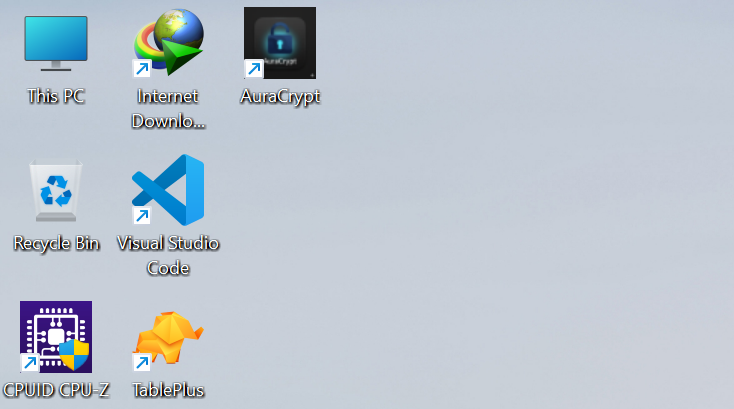
\includegraphics[width=0.6\textwidth]{images/desktop_shortcut_final.png}
    \caption{Shortcut AuraCrypt trên desktop Windows}
    \label{fig:desktop_shortcut}
\end{figure}
\newpage